% -*- TeX:de -*-
\NeedsTeXFormat{LaTeX2e}
\documentclass[12pt,a4paper]{article}
\usepackage[german]{babel} % german text
\usepackage[DIV12]{typearea} % size of printable area
\usepackage[T1]{fontenc} % font encoding
%\usepackage[latin1]{inputenc} % most likely on Windows
\usepackage[utf8]{inputenc} % probably on Linux
\usepackage{multicol}

% PLOTTING
\usepackage{pgfplots} 
\usepackage{pgfplotstable}
\usepackage{url}
\usepackage{graphicx} % to include images
\usepackage{tikz}
\usepackage{subfigure} % for creating subfigures
\usepackage{amsmath} % a bunch of symbols
\usepackage{amssymb} % even more symbols
\usepackage{booktabs} % pretty tables

% a floating environment for circuits
\usepackage{float}
\usepackage{caption}

%\newfloat{circuit}{tbph}{circuits}
%\floatname{circuit}{Schaltplan}

% a floating environment for diagrams
%\newfloat{diagram}{tbph}{diagrams}
%\floatname{diagram}{Diagramm}

\selectlanguage{german} % use german

\begin{document}








%%%% TO DO
%
% - - Shorty:
%

% - - Patrick
%




%%%%%%% DECKBLATT %%%%%%%
\thispagestyle{empty}
			\begin{center}
			\Large{Fakultät für Physik}\\
			\end{center}
\begin{verbatim}


\end{verbatim}
							%Eintrag des Wintersemesters
			\begin{center}
			\textbf{\LARGE WS 2013/14}
			\end{center}
\begin{verbatim}


\end{verbatim}
			\begin{center}
			\textbf{\LARGE{Physikalisches Praktikum\\ für das Bachelorstudium}}
			\end{center}
\begin{verbatim}




\end{verbatim}

			\begin{center}
			\textbf{\LARGE{PROTOKOLL}}
			\end{center}
			
\begin{verbatim}





\end{verbatim}

			\begin{flushleft}
			\textbf{\Large{Experiment (Nr., Titel):}}\\
							%Experiment Nr. und Titel statt den Punkten eintragen
			\LARGE{PW5 Gasthermometer, Adiabatenkoeffizienten, Dampfdichte}	
			\end{flushleft}

\begin{verbatim}

\end{verbatim}	
							%Eintragen des Abgabedatums, oder des Erstelldatums des Protokolls
			\begin{flushleft}
			\textbf{\Large{Datum:}} \Large{07.11.2013}
			\end{flushleft}
			
\begin{verbatim}
\end{verbatim}
							%Namen der Protokollschreiber
		\begin{flushleft}
			\textbf{\Large{Namen:}} \Large{Patrick Braun, Johannes Kurz}
			\end{flushleft}

\begin{verbatim}


\end{verbatim}
							%Kurstag und Gruppennummer, zb. Fr/5
			\begin{flushleft}
			\textbf{\Large{Kurstag/Gruppe:}} \Large{DO/2}
			\end{flushleft}

\begin{verbatim}



\end{verbatim}
							%Name des Betreuers, das Praktikum betreute.
			\begin{flushleft}
			\LARGE{\textbf{Betreuer:}}	\Large{ Franz Sachslehner }	
			\end{flushleft}

%%%%%%% DECKBLATT ENDE %%%%%%%
\pagebreak
\setlength{\columnsep}{20pt}
\begin{multicols}{2}

%%%%%%%%%%%%%%%%%%%%%%%%%%%%%%%%%%%%
\section{Gasthermometer}


\begin{figure}[H]
	\centering
	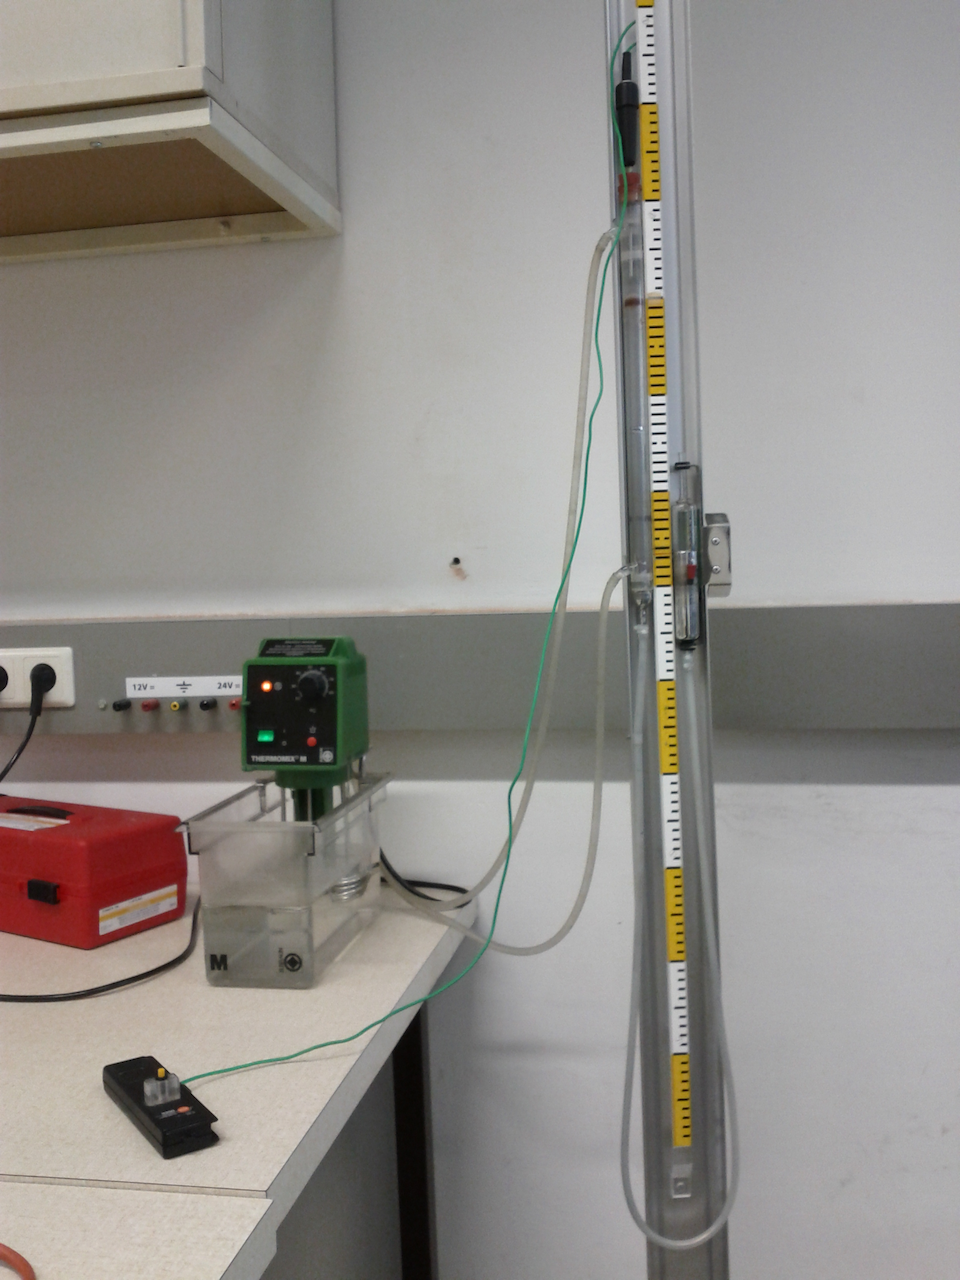
\includegraphics[scale=0.22]{./figure/gas_therm_aufbau.png}
	\caption{Versuchsaufbau mit Heizgerät und Thermometer}
	\label{fig:gas_therm_aufbau}
\end{figure}

%Equipment:
%\begin{itemize}
%	\item[-] Testoterm Sekundenthermometer (9200)
%	\item[-] Halterung mit Quecksilbergefüllten Röhren (siehe Abb. \ref{fig:gas_therm_aufbau} rechts)
%	\item[-] Heizgerät Thermomix B.Braun
%\end{itemize}

\subsection{Messwerte und Ergebnisse}
Luftdruck im Labor: $(993\pm 1)$mBar\\
Raumtemperatur: $(22 \pm 1)^\circ $C


\begin{figure}[H]
	\centering
	\pgfplotstabletypeset[
			columns={Druck, Laenge, Produkt, Fehler},
			%columns/Druck/.style={column name=$Druck\\[mmHg]$},
			col sep=&,
			every head row/.style={before row=\hline,after row=\hline\hline},
			every last row/.style={after row=\hline},
			every first column/.style={
								column type/.add={|}{}
							        },
			every last column/.style={
								column type/.add={}{|} 
								}
			]{
			Druck & Laenge & Produkt & Fehler
			%[mmHg] \pm1; [mm] \pm1; [mmHg*mm]; [mmHg*mm]
			917 &213 &195280 &950 
			794 &229 &181780 &830 
			745 &245 &182480 &790 
			713 &256 &182480 &760
			681 &266 &181090 &740 
	}
	\caption{Messung der Fallzeiten}
	\label{fig:visko_fallzeit}
\end{figure}


\begin{figure}[H]
	\centering
	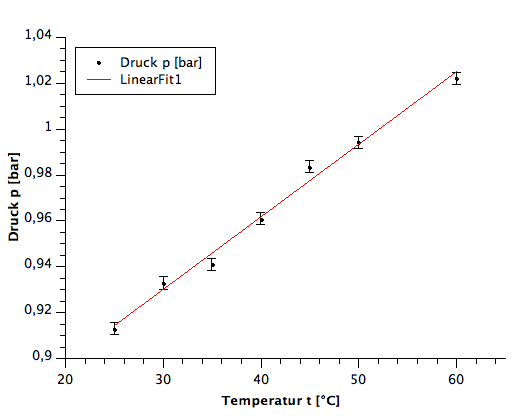
\includegraphics[scale=0.50]{./figure/Spannungskoeffizient-lin_Fit.png}
	\caption{Temperatur gegen mmHg-Differenz, linearer Fit}
	\label{fig:gas_therm_Spannungskoeffizient}
\end{figure}
%B (y-intercept) = 8,350436459016395e-01 +/- 3,812549620209208e-03
%A (slope) = 3,164236065573769e-03 +/- 9,031174786969129e-05

$$\frac{\Delta p}{\Delta \vartheta} = (3.164 \pm 0.091) mbar/ ^\circ C$$
$$ p_0 = (835.0 \pm 3.9) mbar$$\\
\\
$$\beta = (0.00379 \pm 0.00012) K^-1$$
$$T_0 =(263.9 \pm 8.0)K$$



\subsection{Diskussion}




%%%%%%%%%%%%%%%%%%%%%%%%%%%%%%%%%%%%
\section{Adiabatenkoeffizienten der Luft}

%Equipment:
%\begin{itemize}
%	\item[-] Stoppuhr
%	\item[-] Versuchsaufbau mit Pumpe und Metallkugel in Röhre
%\end{itemize}
%
\subsection{Messwerte und Ergebnisse}
Masse Kugel: $(16.828 \pm 0.005)g$ \\
Zwei Messungen, Kugel mit Papier, nur Papier => zwei mal Messfehler.\\

\subsection{Diskussion}



%%%%%% Dampfdichtebestimmung %%%%%%%%

\section{Dampfdichtebestimmung}



\subsection{Messwerte und Ergebnisse}



\subsection{Diskussion}



\section{Quellen}


\end{multicols}
\end{document}